\documentclass[12pt]{report}
\usepackage{enumerate}
\usepackage{hyperref}
\usepackage{times}
\usepackage{apacite}
\usepackage{graphicx}
\graphicspath{{Images/}}

\title{
\includegraphics[scale=1.5]{mmuLogo.jpg}
\\ \\ \\Cyberprotection in IoT environments: A dynamic rule-based solution to defend smart devices} 
\author{Cybersecurity\\\\TPT1201 Research Methodology in Computer Science\\Assignment 1\\ \\Adriana Syaffiya binti Ahmad Khadri \\ 1191200471 \\ \\2423 words}
\date {September 2022}


\begin{document}
%coverpage
\maketitle
%Introduction
\section{Introduction}
A "smart home" has IoT devices that communicate with distant web servers and give users IoT services. Malevolent actors seek to obtain private data and violate the confidentiality, integrity, or availability of such users' data. Smart homes are one of the most prevalent IoT contexts.
\\ \\
IoT security proposals need to be able to dynamically adapt to changes in the scenario. Underprotection and overprotection scenarios, where insufficient or excessive amounts of resources are used, should be avoided. Security proposals for smart homes should focus on providing non-intrusive protection that encourages adoption based on usability.
\\ \\
Security proposals must be able to safeguard digital assets inside of smart home appliances with little to no user involvement while still ensuring that the user is aware of the overall security condition. This is especially important for smart homes as typical users have little experience with IoT management skills.

%Problem Statement and Objectives
\section{Problem Statement and Objectives}
COSMOS does not take into account adaptation to the dangers in the scenario and lacks computational efficiency. The objective of this study is to improve and optimise the COSMOS framework to enable flexible deployment in devices with limited resources while maintaining the protection of IoT devices. The following objectives are defined to accomplish this goal:

\begin{itemize}
\setlength{\itemsep}{-5pt}
\item To keep an eye on the nearby IoT services and devices that are in use, and quickly detect any potential vulnerabilities they may have exposed.
\item To adapt the sentinel dynamically to changes in the nearby smart devices or services, implementing rules appropriate for potential newly discovered security defects to consistently provide the highest level of protection.
\item To construct a mechanism that enables the formulation of dynamic mitigation rules using information about the risks that have been discovered, and then enforce those rules within the thought of a smart scenario
\end{itemize}

%Literature review
\section{Literature Review}
\indent
\cite{Nobakht} proposed a host-based Intrusion Detection and Mitigation framework named IoT-IDM. This proposal concentrates on home use cases and makes use of Software Defined Network (SDN) technology via an SDN controller, which enables network visibility and offers freedom to build, administer, and secure the network remotely. Additionally included are machine learning (ML) approaches for spotting abnormal network behaviour and intrusions. Nevertheless, this technique is not adaptive to changes. \\

\cite{Vakakis} proposed deep learning techniques to guarantee cyber safety in smart home/office scenarios. Two anomaly detection models based on Long-Short Term Memory (LSTM) neural networks are developed. The first model for detecting anomalies focuses on the characteristics of MQTT (Message Queuing Telemetry Transport) traffic that is moving through smart homes and offices. The second one measures total apparent power using sensors and smart devices that have been deployed. Advantage of utilising this technique is it requires no additional management and does not require any computational performance measures. Nevertheless, this technique still suffers from lacking adaptive changes and has no mitigation of the attack.\\

\cite{Anthi} proposed a technique, which is a novel proposal able to predict malicious behaviour and detect malevolent IoT nodes. This proposal uses a machine learning model to learn the behaviour of an IoT-based network. It recognises attacks like network probing and SYN/UDP flood attacks. This proposal also includes a rule-based component that is established in accordance with the security policy. Advantage of utilising this technique is it requires no additional management and does not have any defined main infrastructure required. Nevertheless, this technique has no mitigation of the attack and is not adaptive to changes.\\

\cite{Godquin} proposed a technique, in which the selection of the node where security services should be deployed inside an IoT network is performed using graph theory. Its core technique is to use a weight graph using device capabilities. It takes into account the devices' abilities to create a weighted graph and identify the dominant set, allowing the best place to set up a security service to be determined. The advantage of utilising this technique is it is adaptable to devices’ capabilities. Nevertheless, this technique has no mitigation of the attack.\\

\cite{Brown} proposed a human-in-the-loop artificial immune system for intrusion detection in IoT. The IoT nodes that have been taught to alert users when malicious traffic is present are referred to in this proposal as detectors. The advantage of utilising this technique is it is adaptable to new network traffic. Nevertheless, this technique still suffers from a lack of mitigation of the attack, requires human manual confirmation and requires IoT nodes as it’s the main infrastructure.\\ 



\section{Research Methodology}

\subsection{COSMOS proposal}
ML enforces mitigations with the least amount of latency. The goal of this paper is to suggest a computationally effective solution. It offers an adaptive and dynamic rules management methodology that, in conjunction with an ML module, adapts itself to previously unknown attacks. Such a proposal's primary objective is to defend IoT devices using various defensive mechanisms that follow a strong cyber defence strategy. In Fig. 1, the COSMOS architecture is shown. \\
\begin{center}
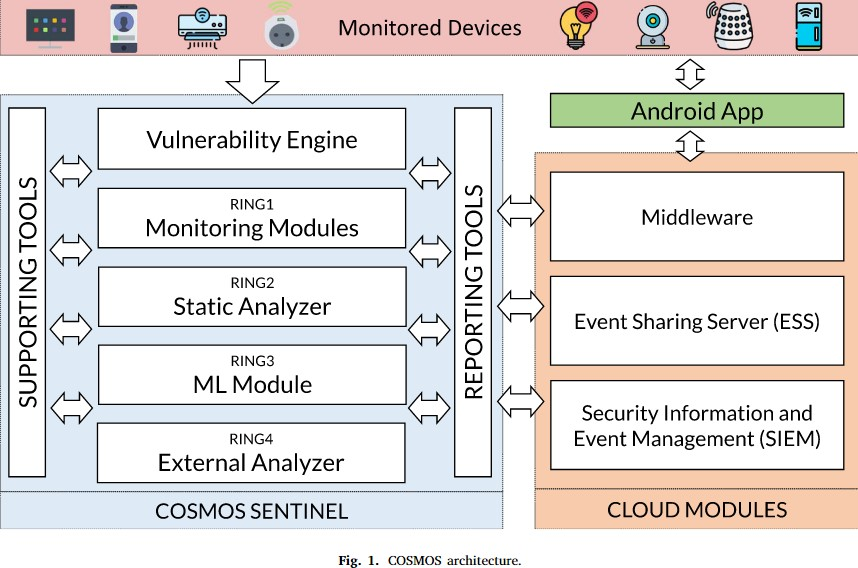
\includegraphics[scale=0.6]{Fig1.jpg}\\
\end{center}

\subsection{Proposed Architecture}
The major goal of this section is to examine and justify the improvements made and how they affect the overall performance and behaviour of the framework after a brief examination of how the various COSMOS components interact and communicate to carry out the protection responsibilities.
\\ \\
This module was broken into several smaller components, one for each distinct purpose. According to the authors, the suggested framework is modular, easily expandable, and easier to maintain in the future. Fig. 2 shows how the system has changed as a result of the addition of new modules. Four additional rules were added. These include Dynamic Rule Loader (DRL), Vulnerability Detection System (VDS), Event Processing Module (EPM), and Mitigation Module (MM). The Scheduler (SCH) component has been introduced to plan a cron job to update the YARA and Suricata rule databases.

\begin{center}
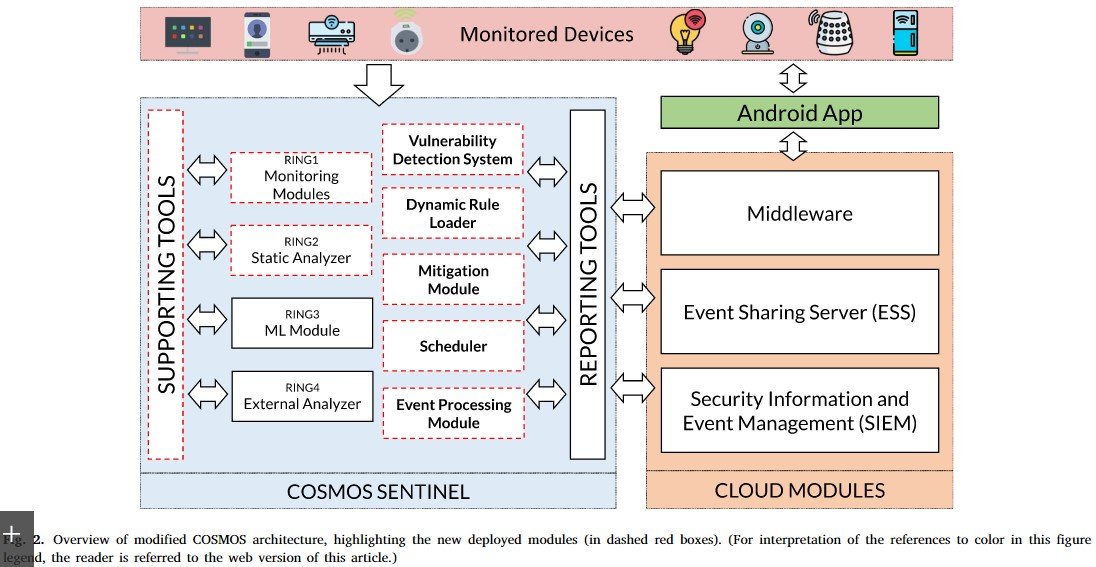
\includegraphics[scale=0.5]{Fig2.jpg}\\
\end{center}
\noindent
The monitoring modules are in charge of intercepting the frames that are moving across the monitored network and then doing a local analysis of them utilising potent IDS rule-based engines. The Ethernet monitor (i.e., Suricata) and the Wi-Fi monitor are deployed as two modules in the proposed architecture (i.e., Kismet). The static analyzer is in charge of utilising robust static analysis algorithms to examine the dangerous samples detected by the monitoring modules and look for potential malware signatures. It serves as the second ring of defence in the suggested framework against potential cyber threats. For the vulnerability detection system, OpenVAS7 (the chosen vulnerability scanner) has a key responsibility: it must scan for and find vulnerabilities in the nearby IoT devices or services that are part of the smart network.
\\ \\
The Scheduler is an essential component of the suggested architecture because it is made to handle operations that must be repeated repeatedly over time, such as vulnerability scanning and updating the IDS and static analyzer rules. For the supporting tools, when used by the other COSMOS sentinel components, these modules carry out a variety of tasks that support the framework's general operation.
\\ \\
For the dynamic rules loader, an ad-hoc DRL was created and implemented to enable dynamic risk management within the smart environment. The deployment of dynamic rules in the suggested framework is shown in Fig. 3

\begin{center}
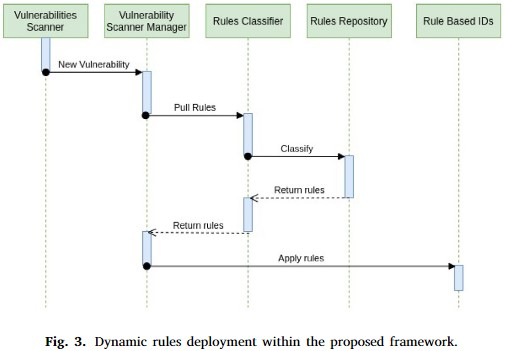
\includegraphics[scale=1]{Fig3.jpg}\\
\end{center}

\noindent
The event processing module analyses all events produced by the IDS and only retains alert-type events that are deemed relevant to our context. Due to its ability to emphasise only the crucial activities taking place in the secured network, such a component is likewise of significant value within the suggested framework. Although it is quite strong, the mitigation module used in this framework has a high level of simplicity. Fig. 4 depicts a quick view of the mitigation procedure flow.

\begin{center}
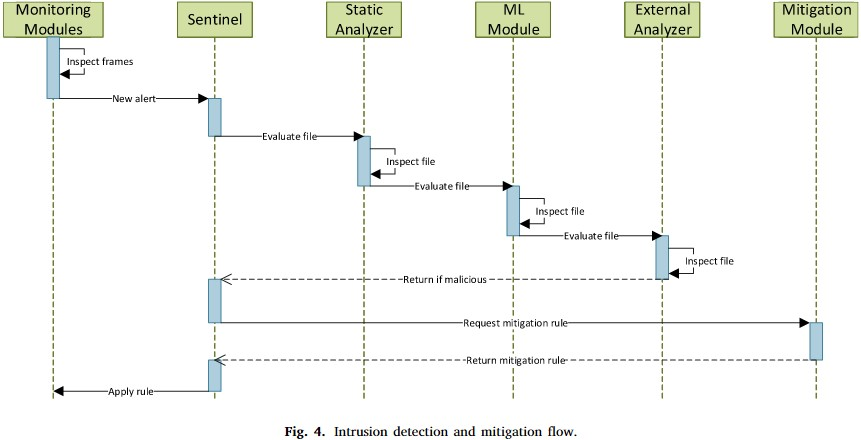
\includegraphics[scale=0.6]{Fig4.jpg}\\
\end{center}

\noindent
Two scenarios were created so that it would be feasible to debate whether the COSMOS framework has improved from its last iteration.
\begin{itemize}
\setlength{\itemsep}{-5pt}
\item Scenario 1: The first scenario is carrying out the trials and loading a complete ruleset into COSMOS.
\item Scenario 2: The second scenario entails reproducing the tests from scenario 1 while also allowing the dynamic rules mechanism to enable measurement of the effects of the defined strategy on COSMOS performance and operations.
 \end{itemize}
The stages that described the experiments are then presented in both cases:
\begin{enumerate}[1.]
\setlength{\itemsep}{-5pt}
\item Prepare a smart home scenario.
\item Deploy COSMOS to protect the smart home.
\item Startup COSMOS modules.
\item Expose vulnerabilities in the smart home scenario.
\item Measure the behaviour of COSMOS through the defined metrics.
\end{enumerate}
These vulnerabilities are described in further detail after this:
A downstream traffic containing malicious files.
\begin{itemize}
\setlength{\itemsep}{-5pt}
\item An Apache HTTP server (2.4.18) exposes the 80 port which serves the previously mentioned malicious files.
\item A web console for Apache ActiveMQ with pre-configured login information.
\item A SSL/TLS protocol utilisation without HTTP Strict Transport Security (HSTS).
\item A MQTT Broker without authentication
 \end{itemize}
These malicious files were used to test COSMOS's ability to keep an eye on the smart home network, find security vulnerabilities in the surrounding area, and reduce the risk that was about to emerge. The COSMOS ruleset for both scenarios was constructed using the 55,718 rules from Emerging Threats. Each test lasted for 120-200 s.

%Performance Evaluation 
\section{Performance Evaluation}
\noindent
The proposed version of COSMOS conducts an accurate and quick detection across the various protection layers with a discernible improvement, according to experimental data. The IDS (also known as Suricata) had the greatest improvement in RAM usage, with an average reduction of 500 MB. The authors improved the rate of IDS dropped and analysed packets by the second-highest amount possible. Because the enhanced IDS uses a lot fewer rules to compare incoming traffic, authors were able to achieve better CPU efficiency with lower CPU consumption peaks. Additionally, COSMOS was able to handle more packets, increasing its detection capacity and giving the smart appliance's intelligent devices constant cyber protection. Because it can handle more packets than the prior version, this approach improves performance in terms of resources used and detection quality. 
\\ \\
Due to the additional processing power required to keep in memory the complete status of the surrounding scenarios, the sentinel core modules were also requiring more RAM than the prior version. In contrast to the prior version, when the whole ruleset was used to maintain precise performance in detection, the new dynamic rule management significantly reduces resource use. Because COSMOS examined a significantly greater number of packets, its ability to process traffic was enhanced. 
\\ \\
Figure 5(a) displays the CPU usage for the chosen IDS in scenarios 1 and 2. (i.e., Suricata). More precisely, Fig. 5(a) shows many CPU peaks near 100\% in scenario 1 (i.e., the IDS employing the complete ruleset). Instead, in case 2, it never exceeds 40\% of CPU consumption, which is a significant improvement. Additionally, Fig. 5(b) shows how much RAM is used for the chosen IDS in both situations 1 and 2. (i.e., Suricata). Since the whole ruleset is loaded in scenario 1 to address the risks within the smart network, the RAM usage exceeds 600 MB in that scenario. However, by using dynamic rule management, the RAM use is improved by 83\%, dropping to 100 MB at its peak..
\begin{center}
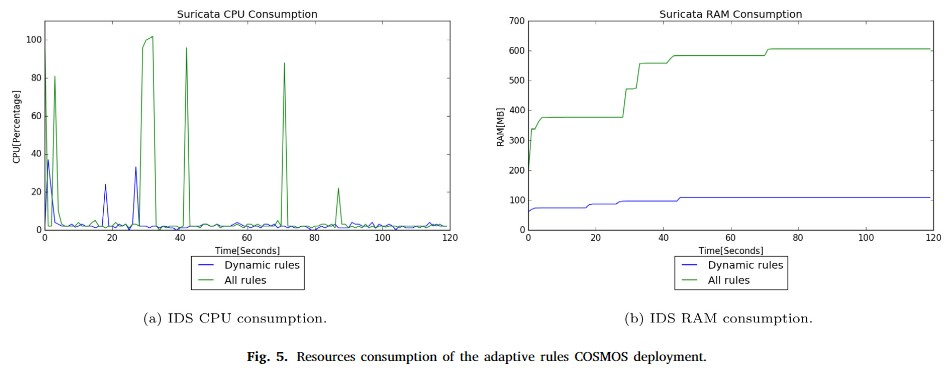
\includegraphics[scale=0.6]{Fig5.jpg}\\
\end{center}
\noindent
It is significant to note that experiments were conducted repeatedly in order to prevent interference and potential out-layers. Nevertheless, there were minimal or no variances in the results. In scenario 2 executions, COSMOS was reliable and capable of finding every vulnerability while modifying the loaded rule set as needed.
\\ \\
The authors provided an updated and enhanced version of COSMOS [7], a cutting-edge framework to safeguard IoT environments from cyber threats, making it flexible to risk scenarios without sacrificing its ability to cyber-protect IoT devices. This improvement was made possible by making COSMOS aware of the existing weaknesses and exposures in the surrounding smart network and constantly modifying its rule set to the situation. The COSMOS resource usage was optimised thanks to the adaptive technique.
\\ \\
Extensive experiments have been carried out to show the viability and the resulting improvement of the suggested framework. The sentinel and the IDS were put under a lot of strain during the aforementioned tests by several malicious frames that replicated two common attack scenarios to better show off the framework's advancements. Experimental findings show that the modifications made to the COSMOS design significantly enhance both security and performance.

% Claimed Contribution 
\section{Claimed Contribution}
\noindent
Extensive experiments have been carried out to show the viability and the resulting improvement of the suggested framework. The sentinel and the IDS were put under a lot of strain during the aforementioned tests by several malicious frames that replicated two common attack scenarios to better show off the framework's advancements. Experimental findings show that the modifications made to the COSMOS design significantly enhance both security and performance.
\\ \\
The results of the experiments demonstrate that scenario 2 had lower CPU, RAM, and dropped packet usage than scenario 1. Additionally, because COSMOS was able to examine a significantly greater number of packets, its ability to process traffic was enhanced. These advancements imply that COSMOS might be used in the future on hardware with less processing capacity while ensuring an appropriate level of safety for a smart situation.


% Future Work
\section{Conlusion \& Future Work}
\noindent
Cyberattacks on Internet of Things (IoT) devices are becoming more sophisticated and common. The IoT ecosystem faces several security difficulties that call for creative solutions to address the problem. Cyberattacks on IoT devices are likely to be a major cause of concern in the near future. By optimising the code used, for example, in the rule representation, COSMOS implementation could yet be made to be more computationally effective.
\\ \\
As future works, the authors intend to install COSMOS in a programmable home router to test its performance on hardware with actual domestic computational constraints. Future research will focus on methods to link the detected vulnerabilities to the set of available rules. Finally, to assess COSMOS' ability to defend weak IoT environments, the authors intend to design additional trials that incorporate more sophisticated threats

%References
\bibliographystyle{apacite}
\bibliography{myBib}{}
\url{https://www.kismetwireless.net/}
\\ \\
\url{https://suricata-ids.org}
\end{document}

